\documentclass{standalone}
\usepackage{tikz}
\usepackage{xcolor}
\usetikzlibrary{positioning}
\newcommand{\w}[1]{\texttt{W(#1)}}% go Withdraw(#1)
\definecolor{r1}{RGB}{68,119,170}
\definecolor{r2}{RGB}{238,102,51}
\definecolor{w3}{RGB}{34,136,51}


\begin{document}
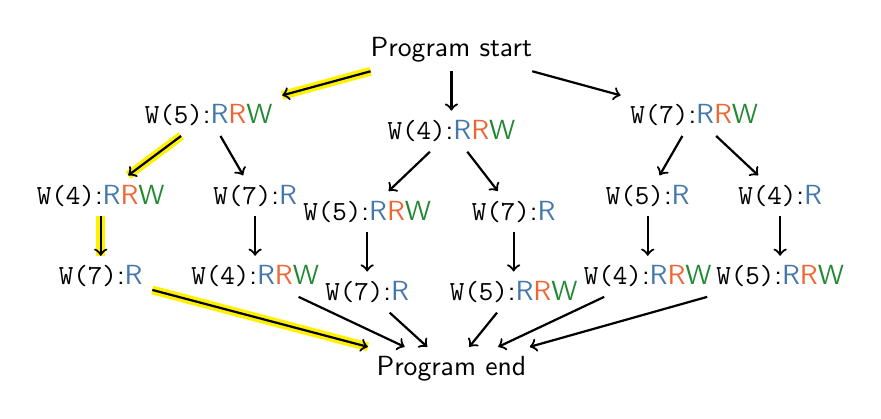
\begin{tikzpicture}[%
  arr/.style={->,thick},%
  glow/.style={preaction={draw,yellow,-,double=yellow,double distance=2\pgflinewidth}}%
  ]
  \node (s) {\sf Program start};
%
  \node (1-5) [below left =0.3 and 1 of s]{\sf\w{5}:\textcolor{r1}{R}\textcolor{r2}{R}\textcolor{w3}{W}};
  \node (1-4) [below      =0.5       of s]{\sf\w{4}:\textcolor{r1}{R}\textcolor{r2}{R}\textcolor{w3}{W}};
  \node (1-7) [below right=0.3 and 1 of s]{\sf\w{7}:\textcolor{r1}{R}\textcolor{r2}{R}\textcolor{w3}{W}};
%
  \node (2-1-4) [below left =0.5 and -0.5 of 1-5]{\sf\w{4}:\textcolor{r1}{R}\textcolor{r2}{R}\textcolor{w3}{W}};
  \node (2-1-7) [below right=0.5 and -1   of 1-5]{\sf\w{7}:\textcolor{r1}{R}};
  \node (2-2-5) [below left =0.5 and -0.8 of 1-4]{\sf\w{5}:\textcolor{r1}{R}\textcolor{r2}{R}\textcolor{w3}{W}};
  \node (2-2-7) [below right=0.5 and -0.8 of 1-4]{\sf\w{7}:\textcolor{r1}{R}};
  \node (2-3-5) [below left =0.5 and -1   of 1-7]{\sf\w{5}:\textcolor{r1}{R}};
  \node (2-3-4) [below right=0.5 and -0.5 of 1-7]{\sf\w{4}:\textcolor{r1}{R}};
%
  \node (3-1-7) [below=0.5 of 2-1-4]{\sf\w{7}:\textcolor{r1}{R}};
  \node (3-1-4) [below=0.5 of 2-1-7]{\sf\w{4}:\textcolor{r1}{R}\textcolor{r2}{R}\textcolor{w3}{W}};
  \node (3-2-7) [below=0.5 of 2-2-5]{\sf\w{7}:\textcolor{r1}{R}};
  \node (3-2-5) [below=0.5 of 2-2-7]{\sf\w{5}:\textcolor{r1}{R}\textcolor{r2}{R}\textcolor{w3}{W}};
  \node (3-3-4) [below=0.5 of 2-3-5]{\sf\w{4}:\textcolor{r1}{R}\textcolor{r2}{R}\textcolor{w3}{W}};
  \node (3-3-5) [below=0.5 of 2-3-4]{\sf\w{5}:\textcolor{r1}{R}\textcolor{r2}{R}\textcolor{w3}{W}};
%
  \node (e) [below=3.5 of s] {\sf Program end};
%
  \draw[arr,glow] (s) -- (1-5);
  \draw[arr] (s) -- (1-4);
  \draw[arr] (s) -- (1-7);
%
  \draw[arr,glow] (1-5) -- (2-1-4);
  \draw[arr] (1-5) -- (2-1-7);
  \draw[arr] (1-4) -- (2-2-5);
  \draw[arr] (1-4) -- (2-2-7);
  \draw[arr] (1-7) -- (2-3-5);
  \draw[arr] (1-7) -- (2-3-4);
%
  \draw[arr,glow] (2-1-4) -- (3-1-7);
  \draw[arr] (2-1-7) -- (3-1-4);
  \draw[arr] (2-2-5) -- (3-2-7);
  \draw[arr] (2-2-7) -- (3-2-5);
  \draw[arr] (2-3-5) -- (3-3-4);
  \draw[arr] (2-3-4) -- (3-3-5);
%
  \draw[arr,glow] (3-1-7) -- (e);
  \draw[arr] (3-1-4) -- (e);
  \draw[arr] (3-2-7) -- (e);
  \draw[arr] (3-2-5) -- (e);
  \draw[arr] (3-3-4) -- (e);
  \draw[arr] (3-3-5) -- (e);
%
\end{tikzpicture}
\end{document}
